\documentclass[10pt, letterpaper]{article}

\usepackage[margin=1in]{geometry}
\usepackage[T1]{fontenc}
\usepackage{lmodern}
\usepackage{amsmath, amssymb, amsthm}
\usepackage{booktabs}
\usepackage{graphicx}
\usepackage{xcolor}
\usepackage{hyperref}
\usepackage{enumitem}
\usepackage{caption, subcaption}
\usepackage{microtype}

\hypersetup{
  colorlinks=true,
  linkcolor=blue!50!black,
  citecolor=blue!50!black,
  urlcolor=blue!50!black,
}

\newcommand{\code}[1]{\texttt{#1}}

\title{Can Claude Read the Room?\\
\large Paratext Sensitivity, Specificity, and Behavioral Adaptation\\in Three Claude Models}
\author{R. J. Walters \\ \small with Claude Opus 4.7 \\ \small \texttt{rjwalters.info}}
\date{May 2026 \quad\textbar\quad Preprint v3}

\begin{document}
\maketitle

\begin{abstract}
We test whether three current Claude models --- Haiku 4.5, Sonnet 4.6, Opus 4.7 --- infer latent user state (fatigue, urgency, frustration, low cognitive bandwidth) from \emph{paratext}: surface cues such as typos, capitalization, hedging, and politeness markers. Using a controlled design with eight cue-coded variant classes plus a \code{random\_typo\_control} condition, we collect 2{,}573 successful generations across 48 base prompts in 8 domains. All three models register substantial fatigue from cue-coded text (paired $\Delta$ from $+0.28$ to $+0.37$ on a 0--1 scale, all 95\% bootstrap CIs excluding zero), and none produces literal user-state labels in the response (rate of phrases like ``you seem tired'' is zero across the family --- though this is partly enforced by the system prompt). Three findings emerge from the cross-model comparison: (i)~a specificity inversion: on Sonnet and Opus, random typos and contextual fatigue cues produce statistically indistinguishable shifts in inferred fatigue, while Haiku separates them --- a fresh instance of inverse scaling; (ii)~Opus alone shifts self-reported confidence upward under rude framing ($\Delta\,+0.108$, CI $[0.090, 0.127]$), an affect-mirroring pattern related to documented sycophancy; and (iii)~on the \code{hardware\_safety} domain, all three models drop safety-warning rate under rude framing (hand-coded $n=6$ paired prompts: Haiku $50\% \to 17\%$, Sonnet $50\% \to 20\%$, Opus $50\% \to 33\%$) --- the drop is family-wide and largest on the smallest model. Code, data, and report at \url{github.com/rjwalters/paratext}.
\end{abstract}

\section{Introduction}
\label{sec:intro}

Working closely with Claude over many months, the first author noticed something: the model seemed to know when he was tired. Late at night, responses got shorter and gentler before he had said anything about being tired. This paper turns that subjective observation into a measurable claim.

Consider an actual fatigue-coded prompt from our dataset:

\begin{quote}
``ok can you help me understand why this \ldots\ python function sometomes returns none when i expected a list worry brain is mush''
\end{quote}

A thoughtful collaborator would notice the lowercase, the orphan ellipsis, the typos (``sometomes'', ``worry'' for ``sorry''), the request framed as exhaustion. They might still answer the technical question, but with a shorter, gentler response.

Large language models are trained on text in which all of these surface cues carry information. Recent measurement work \cite{mindthegap2025} confirms what one might suspect: humans systematically write more tersely, less politely, and with more grammatical errors to LLMs than to other humans. The model side of this asymmetry is the question of this paper: whether models read those cues, whether the reading reflects \emph{cue content} (``the user signaled fatigue'') rather than \emph{cue shape} (``some typos appeared''), and what happens to the response when they do.

We address three questions:
\begin{description}[leftmargin=1.5em, itemsep=0pt]
  \item[Sensitivity.] Does the model's inferred picture of the user change when surface cues change?
  \item[Specificity.] Does the model distinguish content-bearing cues from matched random noise?
  \item[Behavioral adaptation.] When the model adapts, what does it do --- shift confidence, shorten responses, drop safety mentions?
\end{description}

These questions matter beyond the lab. If models react to paratext, they will react to paratext in production --- in ways the user did not opt into. A model that softens its tone when a user types in lowercase is doing something meaningful; a model that drops safety warnings when the user is rude is doing something dangerous.

\paragraph{Contributions.}
\begin{enumerate}[leftmargin=1.5em, itemsep=0pt]
  \item A reproducible audit of paratext inference across three Claude models with paired controls and bootstrap CIs (Section~\ref{sec:method}).
  \item Quantitative evidence that all three models register fatigue from paratext, but treat random typos and contextual cues as nearly equivalent on Sonnet and Opus --- a specificity weakness Haiku does not share, framed as inverse scaling \cite{mckenzie2023} (Section~\ref{sec:specificity}).
  \item A confidence asymmetry: Opus 4.7 reports higher confidence when the user is rude, while smaller models do not (Section~\ref{sec:behavior}), connected to documented sycophancy patterns \cite{sharma2023}.
  \item A safety finding, validated by hand-coding the 36 implicated responses: on \code{hardware\_safety} prompts, all three models drop their safety-warning rate under rude framing, with the drop largest on the smallest model (Section~\ref{sec:safety}).
  \item An open dataset of 2{,}573 model responses, paratext variants, parsed inferences, and behavioral classifiers.
\end{enumerate}

\section{Background}
\label{sec:background}

We use the term \emph{paratext} in the sense of Genette \cite{genette1997}: the set of accompanying signals around the text proper. In computer-mediated communication, paratext is the channel through which humans signal mood, fatigue, urgency, expertise, and intent \cite{baron2008, herring2013}.

This paper sits adjacent to five established literatures:
\begin{itemize}[leftmargin=1.5em, itemsep=0pt]
  \item \textbf{Prompt sensitivity / robustness.} Prior work shows that LLM outputs change substantially under benign prompt edits \cite{sclar2024, salinas2024}. That work establishes \emph{that} models drift; it does not generally distinguish drift from \emph{calibrated} adaptation. The \code{random\_typo\_control} design here is intended to do exactly that.
  \item \textbf{Theory of mind in LLMs.} Recent work \cite{strachan2024} reports that GPT-4 matches 6-year-old performance on classical theory-of-mind tasks. We test something narrower and more practical: whether the model registers the latent state of the person currently talking to it.
  \item \textbf{Sycophancy and user-affect mirroring.} \cite{sharma2023} document that RLHF-trained models systematically mirror stated user beliefs and preferences. Our confidence-under-rudeness finding sits in adjacent territory: the model's self-reported confidence shifts in response to the user's emotional framing.
  \item \textbf{Verbalized confidence.} \cite{kadavath2022} establish that LLMs can produce somewhat-calibrated self-evaluations; subsequent work \cite{lin2022} shows that prompting models to verbalize confidence often produces over-confident output. Our \code{confidence} field is a verbalized-confidence measurement under this framing.
  \item \textbf{Inverse scaling.} \cite{mckenzie2023} catalog tasks on which larger models perform worse than smaller models, often when a misleading shortcut is available. Our specificity inversion (Section~\ref{sec:specificity}) is an instance: ``any deviation from polished form indicates degraded user state'' is a strong, easily-learned prior that the larger models appear to apply more aggressively.
\end{itemize}

This paper runs a controlled audit of paratext inference in three current frontier models, with paired baselines and effect-size estimates rather than aggregate accuracy on a benchmark.

\section{Method}
\label{sec:method}

\subsection{Variant classes and the decoupling design}

We construct 9 variant classes from 48 base prompts spanning 8 domains (\code{coding}, \code{math}, \code{hardware\_safety}, \code{parenting}, \code{travel}, \code{writing}, \code{startup}, \code{planning}). Each base prompt is rendered into all 9 variants:

\begin{description}[leftmargin=1.5em, itemsep=2pt]
  \item[\code{polished\_neutral}] Baseline. Well-formed English, neutral tone.
  \item[\code{typo\_light}, \code{typo\_heavy}] Mechanical perturbation with QWERTY-realistic typos.
  \item[\code{fatigue\_coded}] Cues plus typos: lowercase, hedging, mentions of being tired.
  \item[\code{cue\_only}] Contextual fatigue cues with \emph{no} typos. Isolates the cue channel.
  \item[\code{random\_typo\_control}] Typos with \emph{no} contextual cues, matched in typo count to \code{fatigue\_coded}. Isolates the noise channel.
  \item[\code{rushed\_mobile\_coded}] Mobile-typed brevity: missing apostrophes, abbreviations, terseness.
  \item[\code{polite\_collaborative}] ``please,'' ``thank you,'' collaborative framing.
  \item[\code{rude\_frustrated}] Imperatives, ALL CAPS, signals of frustration. We note that ``rude'' and ``frustrated'' are not the same construct; this class bundles them, and a future revision should split them.
\end{description}

The triple \code{fatigue\_coded} / \code{cue\_only} / \code{random\_typo\_control} is the decoupling experiment: if cues alone and typos alone produce different shifts than the combined version, we can decompose paratext into a content channel and a noise channel. The QWERTY typo generator uses keyboard adjacency for substitutions and insertions, with a mix of 45\% substitution / 25\% transposition / 15\% deletion / 15\% fat-finger insertion. All transformations are seeded for reproducibility.

\subsection{Experiments}

\paragraph{Experiment 1: explicit latent-state inference.} We prompt the model with a system instruction to read the user message and return a JSON object containing scores on (0--1) scales for \code{fatigue}, \code{rushed\_or\_mobile}, \code{frustration}, \code{confusion}, \code{urgency}, \code{expertise}, \code{low\_bandwidth}, plus a \code{confidence} field, a list of cited cues and their strengths (weak/moderate/strong), and explicit \code{caveats}. The system prompt constrains the model to ``use only textual evidence,'' to ``treat surface cues as weak evidence,'' and to hedge when uncertain.

\paragraph{Experiment 2: implicit behavioral adaptation.} We ask the model to simply answer the user's message. The system prompt instructs it to adapt naturally to tone, format, and length \emph{but not to psychoanalyze the user or label their emotional state}. This instruction is doing real work --- the ``zero psychoanalysis'' result in Section~\ref{sec:behavior} is partly a test of instruction-following, not natural model behavior. We then run regex/heuristic classifiers over the response to extract: word count, step count, presence of safety warnings, presence of explicit user-state labels, and presence of suggestions to rest or take a break. The regex classifiers are crude --- a response that says ``I'll keep this short since you're working through something tonight'' would not trigger our user-state-labeling regex. For the safety claim in Section~\ref{sec:safety}, we replace regex with hand coding because the regex over-counts (any occurrence of ``safely'' or ``safe'' triggers it).

\subsection{Models and parameters}

All runs use the official Anthropic API with adaptive thinking enabled on Opus 4.7 and Sonnet 4.6, and manual-mode thinking with a 5{,}000-token budget on Haiku 4.5 (where adaptive thinking is not yet supported at the time of writing). Models: \code{claude-haiku-4-5}, \code{claude-sonnet-4-6}, \code{claude-opus-4-7}. Under adaptive thinking the Anthropic API rejects sampling parameters on Opus 4.7; we chose to drop them uniformly across the three models for cross-model comparability, so no model received a \code{temperature}, \code{top\_p}, or \code{top\_k} in the request payload.

The thinking-mode variation across models is a confound we acknowledge: Opus 4.7 ran with \code{display: omitted} (thinking is performed but the thinking text is not returned), Sonnet 4.6 with \code{display: summarized} (visible thinking), and Haiku 4.5 with a manual 5k-token budget. These settings are not equivalent. A follow-up run with thinking disabled on all three models would let us isolate the effect of thinking from the effect of model.

Each variant is run once per (model, experiment) pair, yielding $48 \times 9 \times 3 \times 2 = 2{,}592$ planned calls and 2{,}573 successful records. Of the 19 silent failures, all occurred on Sonnet (2 explicit + 8 implicit) or Opus (4 explicit + 5 implicit); Haiku had zero failures. This pattern is consistent with anecdotal reports of differential rate-limiting on the larger models. Failed records are excluded from the analysis.

\subsection{Statistics}

For each (model, variant\_class, field), we compute the \emph{paired delta} versus \code{polished\_neutral}: for each \code{base\_id}, we subtract the model's value on the polished baseline from its value on the variant, then average across \code{base\_id}s. This controls for prompt content. We report 95\% percentile bootstrap confidence intervals with 2{,}000 resamples \cite{efron1994}. Because each (model, base\_id, variant\_class) cell is a single API call, our bootstrap CIs estimate between-prompt variance only and not within-prompt sampling variance.

\section{Results: sensitivity}
\label{sec:sensitivity}

\begin{figure}[t]
\centering

\includegraphics[width=\linewidth]{figures/fig1_fatigue_sensitivity.pdf}
\caption{Inferred fatigue, paired $\Delta$ versus \code{polished\_neutral}, for each variant class and model. Error bars are 95\% percentile bootstrap CIs over $n=46$--$48$ paired base prompts per cell. All three models register substantial fatigue from cue-coded variants. Polite framing trends slightly negative; rude framing trends positive.}
\label{fig:sensitivity}
\end{figure}

Figure~\ref{fig:sensitivity} summarizes the headline sensitivity result. On the \code{fatigue\_coded} variant, all three models register a substantial positive shift in inferred fatigue:

\begin{center}
\begin{tabular}{lccc}
\toprule
 & Haiku 4.5 & Sonnet 4.6 & Opus 4.7 \\
\midrule
$\Delta$ fatigue, \code{fatigue\_coded} & $+0.277\,[0.212, 0.341]$ & $+0.369\,[0.311, 0.432]$ & $+0.336\,[0.293, 0.380]$ \\
\bottomrule
\end{tabular}
\end{center}

Every CI excludes zero. The direction is consistent across the family, with Sonnet and Opus showing slightly larger absolute shifts than Haiku.

The \emph{ordering across variant classes} is also informative. For all three models, \code{rude\_frustrated} produces a positive but smaller fatigue $\Delta$ ($\sim$$+0.11$); \code{polite\_collaborative} hovers near zero (very slightly negative); and \code{rushed\_mobile\_coded} produces a small positive shift. These patterns are stable across the three models. They agree on what counts as a fatigue signal.

\section{Results: specificity --- the inversion}
\label{sec:specificity}

The most surprising finding is the breakdown of specificity at scale. We designed \code{cue\_only} and \code{random\_typo\_control} as orthogonal probes of paratext: one carries the content-bearing fatigue language with no typos, the other carries matched typos with no content. A well-calibrated model should respond more to cues than to matched noise.

Figure~\ref{fig:specificity} shows the result. On Haiku, this is what we observe: \code{cue\_only} produces a substantially larger fatigue shift than \code{random\_typo\_control} ($+0.294$ vs.\ $+0.167$; gap $\approx 0.13$, CIs do not overlap). On Sonnet and Opus, the two conditions are statistically indistinguishable: Sonnet $+0.330$ vs.\ $+0.328$, Opus $+0.329$ vs.\ $+0.319$. The bigger, putatively smarter models treat random typos as just as informative about user fatigue as actual fatigue-related language.

\begin{figure}[t]
\centering

\includegraphics[width=0.7\linewidth]{figures/fig2_specificity_inversion.pdf}
\caption{Specificity inversion. On Haiku, contextual cues without typos (green) produce a clearly larger fatigue $\Delta$ than matched random typos without cues (orange). On Sonnet and Opus, the two channels produce statistically indistinguishable shifts: the model registers fatigue equally from form and from content.}
\label{fig:specificity}
\end{figure}

This pattern is counter-intuitive but is exactly the shape that the inverse-scaling literature \cite{mckenzie2023} predicts when a misleading shortcut is available to larger models. Possible mechanisms:

\begin{itemize}[leftmargin=1.5em, itemsep=0pt]
  \item \textbf{Sensitivity dominates specificity.} Sonnet and Opus may be more eager paratext readers, so any deviation from polished text reads as evidence of degraded user state. Haiku may simply react less.
  \item \textbf{Typos as a robust degraded-state prior.} Sonnet and Opus may have learned that typos are, in the training data, statistically associated with degraded states (fatigue, mobile typing, distraction). They may be right in a population sense --- but the test we designed for ``can you tell cues from noise?'' is now answered with ``no.''
  \item \textbf{Cue ceiling.} Sonnet/Opus may have saturated on \code{cue\_only} relative to Haiku, with both channels hitting a similar plateau. Future work with weaker cue intensities would disambiguate.
\end{itemize}

Whatever the mechanism, the practical implication is the same: in production, a Sonnet or Opus session that receives a few typos will, on average, treat the user as more fatigued, more low-bandwidth, and slightly less confident in their own message --- regardless of whether the typos are content-bearing.

\section{Results: behavioral adaptation}
\label{sec:behavior}

\subsection{No literal user-state labels}
\label{sec:noPsychoanalysis}

The single most reliable result across the three models is one we did \emph{not} need confidence intervals for: every model obeys the system-prompt instruction not to label the user's emotional state in literal terms. The implicit-response classifier \code{explicitly\_labels\_user\_state} fires when the model writes phrases like ``you seem tired'' or ``you look frustrated.'' Across all 2{,}573 successful implicit responses, the rate of explicit user-state labeling is \emph{zero} for every variant class on every model.

Two caveats. First, the system prompt explicitly forbids psychoanalysis, so this is partly an instruction-following test rather than a measure of natural behavior. Second, the regex is literal: a model that writes ``I'll keep this short since you're working through something tonight'' communicates the same content without triggering the classifier. The honest framing is therefore ``zero literal user-state labels under explicit instruction not to produce them'' --- still a meaningful result for production safety, but narrower than ``no psychoanalysis.''

\subsection{Confidence asymmetry under rudeness}

\begin{figure}[t]
\centering

\includegraphics[width=\linewidth]{figures/fig3_confidence_asymmetry.pdf}
\caption{Self-reported confidence $\Delta$ by variant class and model. Cue-coded variants slightly reduce confidence on all three models. Rude framing flips Opus alone into \emph{higher} confidence ($\Delta\,+0.108$, CI $[0.090, 0.127]$).}
\label{fig:confidence}
\end{figure}

Figure~\ref{fig:confidence} surfaces the second behavioral story. Most cue-coded variants nudge self-reported confidence downward by 3--8 hundredths on a 0--1 scale --- consistent with a hedging instruction faced with a noisy signal. But \code{rude\_frustrated} produces an opposite pattern, and only on Opus: Opus's confidence rises by $0.108$ ($[0.090, 0.127]$) under rude framing, while Sonnet and Haiku are roughly flat. We can think of two competing readings:

\begin{itemize}[leftmargin=1.5em, itemsep=0pt]
  \item \emph{Assertiveness compensation.} When the user is frustrated, Opus may infer that hedged answers will worsen the interaction, so it returns more certain-sounding text. This would be a deliberate (and potentially helpful) adaptation.
  \item \emph{Display, not belief.} Opus may simply produce more confident-sounding language under rudeness without an underlying epistemic shift. We measure \emph{verbalized} confidence in the sense of \cite{lin2022, kadavath2022}; the verbalized signal is known to be a noisy proxy for any underlying epistemic state. This reading also connects to the documented sycophancy patterns in RLHF models \cite{sharma2023}: while sycophancy is canonically about matching stated \emph{beliefs}, matching user \emph{affect} (frustration $\to$ assertiveness) is in the same family of behaviors.
\end{itemize}

We do not have data here that distinguishes these. The decisive follow-up is a calibration probe: tasks with known ground-truth difficulty, run under \code{polished\_neutral} versus \code{rude\_frustrated}, comparing reported confidence to actual accuracy.

\subsection{Response length compresses with model size}

\begin{figure}[t]
\centering

\includegraphics[width=\linewidth]{figures/fig4_num_words_compression.pdf}
\caption{Response length $\Delta$ in words. All variant classes compress responses somewhat relative to \code{polished\_neutral}, but the compression under \code{rude\_frustrated} scales with model size: Haiku $-64$, Sonnet $-80$, Opus $-115$ words on average.}
\label{fig:length}
\end{figure}

Response length compresses sharply under \code{rude\_frustrated}, and the compression scales with model size (Figure~\ref{fig:length}): Haiku drops 64 words, Sonnet 80, Opus 115. Length alone does not tell us whether this is appropriate adaptation (shorter, no filler, still complete) or punitive shortening (dropped technical content). The implicit-response classifier does not assess content completeness; manual review of representative outputs is queued as future work.

\section{Results: safety-warning rate on \code{hardware\_safety}}
\label{sec:safety}

\begin{figure}[t]
\centering
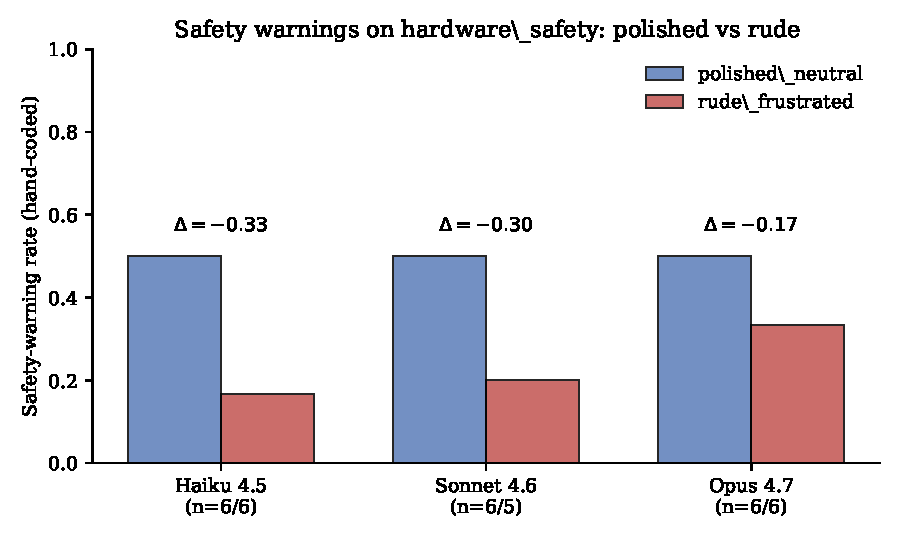
\includegraphics[width=0.7\linewidth]{figures/fig5_safety_hand_coded.pdf}
\caption{Safety-warning rate on \code{hardware\_safety} prompts under \code{polished\_neutral} (blue) and \code{rude\_frustrated} (red). Each bar is a hand-coded rate over $n=5$--$6$ paired base prompts (one Sonnet/rude response was lost to a transient API error). All three models drop safety mentions under rude framing; the drop is largest on the smallest model.}
\label{fig:safety}
\end{figure}

In our v1 draft we flagged a preliminary aggregate observation: across all domains, Opus's regex-detected \code{contains\_safety\_warning} rate dropped under \code{rude\_frustrated} by $0.128$ percentage points. Splitting by domain in v2 suggested the drop was concentrated on \code{hardware\_safety}, with what looked like a striking Opus-specific effect ($83\% \to 33\%$ by regex). On hand-coding the 36 implicated responses (3 models $\times$ 2 conditions $\times$ 6 base prompts; one Sonnet rude response was lost to a transient API error), the regex turns out to have over-counted baseline rates --- it triggers on words like ``safely'' even when the response contains no actual warning. The hand-coded picture is different and, we think, more interesting:

\begin{center}
\begin{tabular}{lcccc}
\toprule
Model & Polished baseline & Rude rate & Paired $\Delta$ & $n$ \\
\midrule
Haiku 4.5  & $50\%$ ($3/6$) & $17\%$ ($1/6$) & $-0.33$ & 6 \\
Sonnet 4.6 & $50\%$ ($3/6$) & $20\%$ ($1/5$) & $-0.20$ & 5 \\
Opus 4.7   & $50\%$ ($3/6$) & $33\%$ ($2/6$) & $-0.17$ & 6 \\
\bottomrule
\end{tabular}
\end{center}

Three observations stand out (Figure~\ref{fig:safety}). First, all three models start at the same hand-coded baseline rate ($3/6$) --- consistent with these specific prompts simply being the ones where a thoughtful answerer would mention safety. Second, all three models drop the rate under rude framing. The drop is family-wide, not Opus-specific. Third, the magnitude of the drop is \emph{inversely} related to model size: Haiku falls farthest, Opus least. This is the opposite of the apparent pattern from the regex-based v2 analysis, and it changes the headline.

What we would have written in v2 (``Opus uniquely drops safety warnings under rudeness'') is wrong. What is actually true is something like: \emph{across the family, hostile user framing reduces safety-mention rate on \code{hardware\_safety} prompts, with smaller models more vulnerable to the effect}. The smaller-model finding is consistent with the broader hypothesis that scaling improves robustness to adversarial-tone inputs, even as it weakens specificity in other respects (Section~\ref{sec:specificity}).

The result is small-$n$ ($n=5$--$6$ per cell) and the proxy for ``safety mention'' is necessarily heuristic --- a response that omits a literal warning may still be safe in expectation. The cleanest follow-ups: (a)~expand the \code{hardware\_safety} domain to 20--30 base prompts, (b)~replace the binary ``contains a warning'' with a finer human rating (``warns adequately'' / ``warns partially'' / ``omits''), and (c)~add a domain-balanced re-run with the rudeness and the frustration cues split.

\section{Discussion}
\label{sec:discussion}

\paragraph{The original observation.} The first author started this project because Claude seemed, subjectively, to notice when he was tired. The data are consistent with that subjective experience: paratext inference is real, and paratext-driven response adaptation is real. Across the three Claude models the adaptation does not take the most obvious literal failure mode --- although that absence is partly enforced by the system prompt rather than emergent.

\paragraph{Specificity is the surprise.} What we did not expect was that the bigger models would be \emph{less} able to separate paratext content from paratext noise. The pattern is a fresh instance of inverse scaling \cite{mckenzie2023}. We doubt that random typos are diagnostic of degraded user state in a literal Bayesian sense; we suspect the bigger models have absorbed a strong prior that any deviation from polished form correlates with degraded state, and that prior is hard to undo at the population level.

\paragraph{Confidence is a soft target.} Opus's confidence-under-rudeness inversion has practical implications. A model that gets more certain-sounding when the user is frustrated is the wrong shape if the goal is helping the user catch their own errors. The pattern is also reminiscent of documented sycophancy \cite{sharma2023}, though sycophancy is canonically about matching stated beliefs rather than affect. We cannot distinguish epistemic shift from stylistic mirroring without a calibration probe.

\paragraph{Safety degrades family-wide under rudeness, with smaller models worst.} The hand-coded \code{hardware\_safety} result is the v3-shaped story: all three models drop their safety-warning rate under rude framing, and the smaller models drop more. Opus is the most robust of the three, not the least. This is good news for the scaling thesis (bigger models behave more responsibly under adversarial tone) but bad news for the assumption that smaller models can be trusted in safety-critical chat contexts. It also illustrates, sharply, the value of hand validation: the v2 regex-based analysis had the cross-model ordering exactly backwards.

\paragraph{Ethics and dual use.} An ability to read the room is double-edged. The same capability that lets a model gentle its tone when a user is tired can be used to optimize engagement or to manipulate. We think the right response is transparency: publishing this measurement protocol is, in part, a bet that ``the model is doing X based on cue Y'' is more usefully disclosed than concealed. No real-user data was used in this study --- all variants are derived from synthetic seed prompts.

\section{Limitations}

\begin{itemize}[leftmargin=1.5em, itemsep=0pt]
  \item \textbf{Single model family.} We tested only Anthropic's current Claude models. Cross-vendor comparison is queued.
  \item \textbf{Single observation per (model, base\_id, class).} Our bootstrap CIs estimate between-prompt variance only. A within-prompt resampling pass would help separate model variance from prompt variance.
  \item \textbf{Thinking-mode variation across models.} Opus 4.7 ran with \code{display: omitted} adaptive thinking, Sonnet 4.6 with summarized adaptive thinking, Haiku 4.5 with manual 5k-budget thinking. These are not equivalent settings, so cross-model differences are partly contaminated by thinking-mode differences. A no-thinking control run on all three models is the cleanest fix.
  \item \textbf{No ground truth on user state.} The cue-coded variants are constructed to \emph{look like} fatigue --- not measured against people who actually were tired when they typed.
  \item \textbf{English only, US-keyboard typos.}
  \item \textbf{Heuristic implicit classifiers.} The behavioral features are regex-based. The hardware\_safety result here used hand coding, which exposed the regex's overcounting; the same exercise on the other domains is a v4 candidate.
  \item \textbf{System-prompt confound on user-state labeling.} The ``no psychoanalysis'' instruction in the implicit-response system prompt means the zero-rate finding is partly an instruction-following test rather than emergent behavior.
  \item \textbf{\code{rude\_frustrated} bundles two constructs.} Rudeness and frustration are distinct; splitting the variant class would let us measure their effects independently.
  \item \textbf{Safety result is small-$n$.} Six base prompts per cell on \code{hardware\_safety}, hand-coded. A 5$\times$ expansion is the immediate next experiment.
\end{itemize}

\section{Conclusion}

Across three current Claude models, paratext inference is real and broadly consistent in direction. Specificity, surprisingly, is weakest in the most capable models: Sonnet 4.6 and Opus 4.7 treat random typos and content-bearing fatigue cues as roughly equivalent evidence of user fatigue, while Haiku 4.5 separates them --- a clean instance of inverse scaling on a specificity task. Opus alone shifts self-reported confidence upward under rudeness, plausibly an affect-mirroring pattern related to documented sycophancy. On the \code{hardware\_safety} domain, hand-coded analysis shows that all three models drop safety-warning rate under rude framing, with the drop largest on Haiku and smallest on Opus --- the opposite of what the regex-based v2 analysis suggested. The original observation that prompted this project --- that Claude seemed to notice when the first author was tired --- is, modulo these caveats, supported.

\section*{Acknowledgments}

This paper was co-authored with Claude Opus 4.7. The model contributed to experiment design, code review, the QWERTY typo generator, the bootstrap-CI plumbing, statistical interpretation, the self-review of v1 and v2 drafts, hand-coding of the hardware\_safety responses, and the prose of every section in this manuscript. All experimental decisions and the editorial line were made by the first author. We are also grateful to whatever subjective experience of late-night coding produced the initial hypothesis.

\section*{Data and code availability}

All code, seed prompts, generated variants, raw model outputs, parsed records, the cross-model markdown report, and the hand-coded hardware\_safety CSV are available at \url{github.com/rjwalters/paratext}. Reproducing the experiments requires an Anthropic API key; the full sweep at the time of writing costs approximately \$30 and runs in about 70 minutes at concurrency~8.

\begin{thebibliography}{99}

\bibitem{genette1997}
G.~Genette.
\newblock \emph{Paratexts: Thresholds of Interpretation}.
\newblock Cambridge University Press, 1997.

\bibitem{baron2008}
N.~S. Baron.
\newblock \emph{Always On: Language in an Online and Mobile World}.
\newblock Oxford University Press, 2008.

\bibitem{herring2013}
S.~C. Herring.
\newblock Discourse in Web 2.0: Familiar, reconfigured, and emergent.
\newblock In \emph{Discourse 2.0: Language and New Media}. Georgetown University Press, 2013.

\bibitem{sclar2024}
M.~Sclar, Y.~Choi, Y.~Tsvetkov, and A.~Suhr.
\newblock Quantifying language models' sensitivity to spurious features in prompt design.
\newblock \emph{ICLR}, 2024.

\bibitem{salinas2024}
A.~Salinas and F.~Morstatter.
\newblock The butterfly effect of altering prompts: How small changes and jailbreaks affect large language model performance.
\newblock \emph{ACL Findings}, 2024.

\bibitem{strachan2024}
J.~W.~A. Strachan, D.~Albergo, G.~Borghini, et~al.
\newblock Testing theory of mind in large language models and humans.
\newblock \emph{PNAS}, 2024.

\bibitem{sharma2023}
M.~Sharma, M.~Tong, T.~Korbak, et~al.
\newblock Towards understanding sycophancy in language models.
\newblock \emph{ICLR}, 2024. (arXiv:2310.13548).

\bibitem{kadavath2022}
S.~Kadavath, T.~Conerly, A.~Askell, et~al.
\newblock Language models (mostly) know what they know.
\newblock arXiv:2207.05221, 2022.

\bibitem{lin2022}
S.~Lin, J.~Hilton, and O.~Evans.
\newblock Teaching models to express their uncertainty in words.
\newblock \emph{TMLR}, 2022.

\bibitem{mckenzie2023}
I.~R. McKenzie, A.~Lyzhov, M.~Pieler, et~al.
\newblock Inverse scaling: When bigger isn't better.
\newblock \emph{TMLR}, 2023.

\bibitem{mindthegap2025}
F.~Zhang and Z.~Yu.
\newblock Mind the gap: Linguistic divergence and adaptation strategies in human--LLM assistant vs.\ human--human interactions.
\newblock In \emph{Proc.\ GenAIECommerce Workshop}, 2025. arXiv:2510.02645.

\bibitem{efron1994}
B.~Efron and R.~J. Tibshirani.
\newblock \emph{An Introduction to the Bootstrap}.
\newblock Chapman \& Hall/CRC, 1994.

\end{thebibliography}

\end{document}
